\section{Beschreibung des User Interface Konzepts}

[Detaillierte Beschreibung des Gesamtkonzepts: Wie wird das Interaktionsverhalten abgebildet? Wieso wurde diese Lösung gewählt? Wie wurden die Personas und Szenarios in der Konzeptausarbeitung berücksichtigt? Welche besonderen Prinzipien wurden bei der Realisierung beachtet?

Darstellung anhand der Abbildungen aller erstellten Wireframes oder Mockups und ggf. der Interaktionsabläufe als Flussdiagramm inkl. Beschreibung bzw. Erläuterung der dahinter stehenden Überlegungen in den folgenden Unterkapiteln. Der Zusammenhang der einzelnen Bildschirmmasken und Interaktionsfluss durch das Programm soll klar hervorgehen.]

\subsection{Desktop Web Interface}

\begin{figure}[htl]
\centering
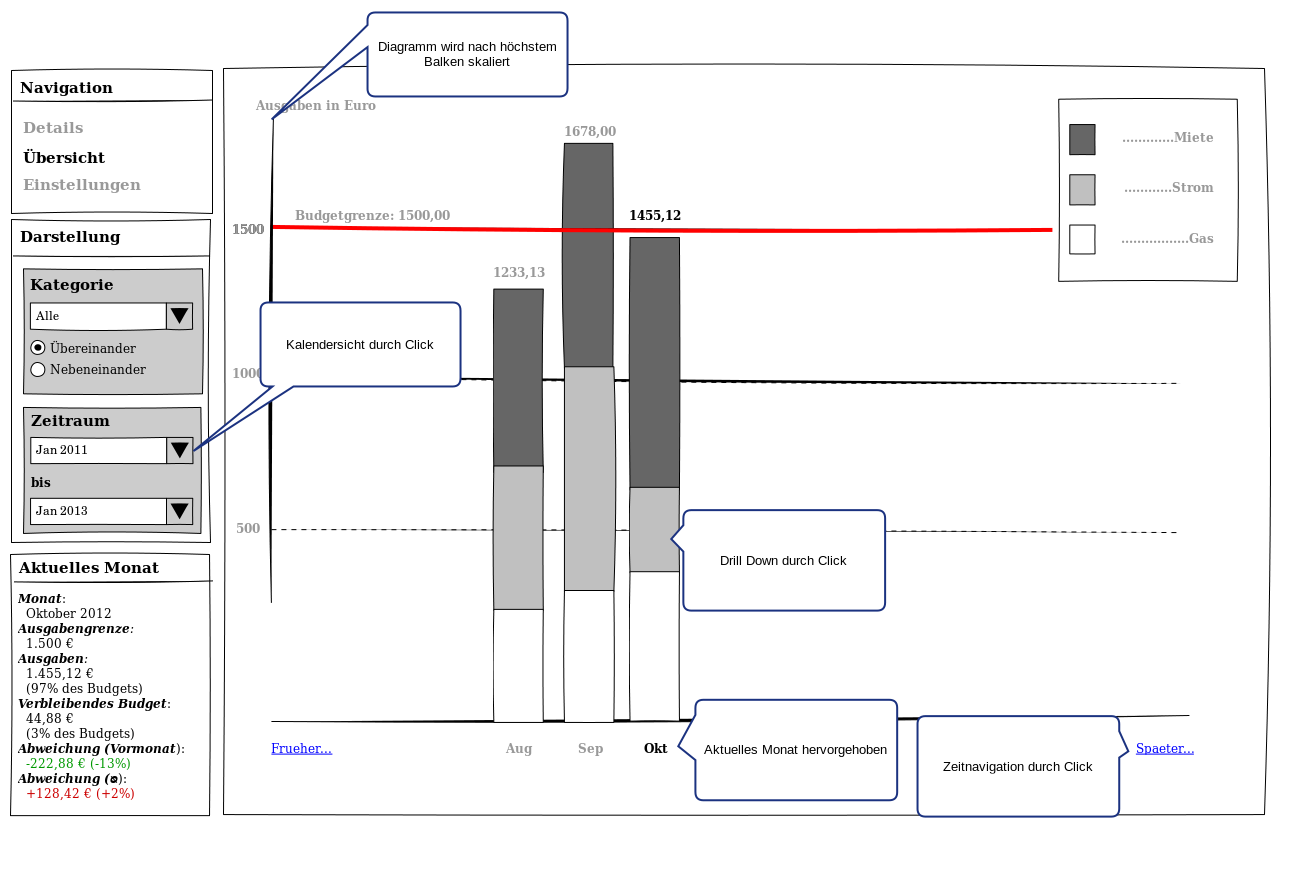
\includegraphics[width=\textwidth]{img/web_uebersicht}
\caption{Web \"Ubersicht}
\label{fig:web_uebersicht}
\end{figure}

\subsection{Mobiles User Interface}
\subsection{Detailfragen}

\subsubsection{Frage 1}

\emph{Wie kann man Benutzer bei der Eingabe von Datensätzen unterstützen? Wie lassen sich Fehleingaben vermeiden? Wie werden diese Konzepte in Ihrem Prototypen realisiert?}

\vspace{2mm}


[Max. 250 Wörter, Wireframes zur Illustration]



\subsubsection{Frage 2}

\emph{Welche Informationen sind für Benutzer besonders wichtig und wie lässt sich deren Bedeutung im System repräsentieren? Welche Such-/Filter-/Sortier-Funktionen sind nützlich?}

\vspace{2mm}

Der Benutzer sollte auf einen Blick alle Ausgaben eines Monats sehen k\"onnen. Diese
werden auf der zentralen \"Ubersichtsseite chronologisch angeordnet dargestellt.

Ebenfalls sind einfache monatliche Zusammenfassungen wichtig; dazu wird in der
\"Ubersichtsseite am Ende jedes Monats eine Zusammenfassungszeile eingeblendet.
Die Zusammenfassung enth\"alt Informationen wie zum Beispiel die Summe aller monatlichen
Ausgaben, dessen Differenz zur festgelegten Budgetgrenze, und Vergleichswerte zu den Ausgaben
anderer Monate. Diese Zeile wird durch Schriftart und Hintergrundfarbe hervorgehoben.
Bei positiver Differenz (Grenze nicht \"uberschritten) ist die Differenz gr\"un dargestellt,
sonst rot.

Eintr\"age, die \"uber die Monatsgrenze hinausgehen werden durch rote Hintergrundfarbe
markiert.

Die Diagramme stellen vor allem Ausgaben pro Monat dar und sind als Balkendiagramme realisiert.
In diesem Zusammenhang ist nat\"urlich die Darstellung der monatlichen Obergrenze wichtig;
diese wird als Linie im Balkendiagramm eingezeichnet. Ebenfalls sind die Proportionen der Kategorien
von Interesse, deshalb wird ein Balken pro Kategorie eingef\"rbt.

Zur \"ubersichtlicheren Darstellung der Entwicklung von einzelnen Kategorien k\"onnen
diese auch in einem gefilterten Diagramm dargestellt werden (andere Kategorien werden
ausgeblendet).



\subsubsection{Frage 3}

\emph{Welche Möglichkeiten gibt es zur graphischen Aufbereitung der Daten (Grafiken, Kalender-Ansicht, etc.)? Wie werden diese Möglichkeiten in Ihrem Prototypen realisiert?}

\vspace{2mm}



[Max. 250 Wörter, Wireframes zur Illustration]



\subsubsection{Frage 4}

\emph{Wie lässt sich eine sinnvolle Aufgabenteilung zwischen Desktop-UI und mobiler UI erreichen? Welche Aufgaben haben bei der Verwendung zu Hause am Schreibtisch die höchste Priorität und welche Aufgaben haben bei der Verwendung am Smartphone die höchste Priorität? Welche Formen der graphischen Aufbereitung sind für den jeweiligen Anwendungskontext angemessen?}

\vspace{2mm}



[Max. 250 Wörter, Wireframes zur Illustration]
